\section{积分的样本估计}
\label{sec:mcerr-estimator}

用随机样本算积分，首先要说清楚算的是什么、用什么去算，以及“误差”指的是哪一个量与哪一个量之差。设$\pi$是取值空间$\mathcal{X}$上的概率分布，$f\colon\mathcal{X}\to\mathbb{R}$可测且$\mathbb{E}_{\pi}\lvert f\rvert<\infty$。要计算的是
\begin{equation}
 I=\mathbb{E}_{\pi}[f]=\int_{\mathcal{X}}f(x)\,\pi(\mathrm{d}x) .
 \label{eq:mcerr-target}
\end{equation}
这里$\pi$与$f$都已完全给定，$I$是一个确定的数，只是不便用公式或网格求积算出。

\paragraph{样本平均}
设某个生成程序产生了$X_1,\dots,X_N$。它们的联合规律由程序决定，称为\emph{实际生成规律}；它可能是$N$个独立的$\pi$样本，也可能各项相关，甚至各项的分布都与$\pi$不同。用函数值的平均
\begin{equation}
 \hat{I}_N=\frac{1}{N}\sum_{i=1}^{N}f(X_i)
 \label{eq:mcerr-estimator}
\end{equation}
近似$I$，这种用随机样本的平均计算积分的方法称为\term{Monte Carlo方法}（Monte Carlo method），$\hat{I}_N$称为$I$的Monte Carlo估计。第~\ref{chap:laws-of-large-numbers}章在四分之一圆的面积上已经用过它。

$\hat{I}_N$中的随机性来自计算过程本身：换一组随机数，结果就会变。这与统计推断不同。统计推断里$\pi$未知，样本是观测到的数据，要由数据推断总体，可参考\BookChapterRef{chap:parametric-statistical-inference}{卷八第1章“参数化统计推断”}。本章的$\pi$是已知的，我们可以随意重新生成样本，问题只在于计算的精度。

\paragraph{偏差与波动}
误差$\hat{I}_N-I$是一个随机变量。设每个$f(X_i)$在实际生成规律下都可积，于是$\mathbb{E}[\hat{I}_N]$有定义，误差可以分成两部分：
\begin{equation}
 \hat{I}_N-I=\underbrace{\bigl(\mathbb{E}[\hat{I}_N]-I\bigr)}_{\text{偏差}}+\underbrace{\bigl(\hat{I}_N-\mathbb{E}[\hat{I}_N]\bigr)}_{\text{随机波动}} .
 \label{eq:mcerr-split}
\end{equation}
第一部分记作$b_N=\mathbb{E}[\hat{I}_N]-I$，称为偏差，它是确定的数，表示重复计算无穷多次以后平均结果离目标多远。第二部分均值为零，表示单次计算围绕自己的平均值摆动多少。$b_N=0$时称$\hat{I}_N$无偏。

偏差只依赖各个$X_i$各自的分布，与它们之间是否独立无关。由期望的线性，
\[
 \mathbb{E}[\hat{I}_N]=\frac1N\sum_{i=1}^{N}\mathbb{E}[f(X_i)] .
\]
所以只要每个$X_i$都服从$\pi$，不论它们怎样相关，$\hat{I}_N$都无偏。反过来，样本之间的依赖只影响第二部分。后面几节正是按这个分工展开的：第~\ref{sec:mcerr-approx}节与第~\ref{sec:mcerr-initial}节处理各项分布偏离$\pi$造成的偏差，第~\ref{sec:mcerr-correlated}节处理依赖对波动的影响。

两部分合在一起时，最常用的尺度是均方误差。

\begin{theorem}[均方误差的分解]
\label{thm:mcerr-mse}
设$\mathbb{E}[\hat{I}_N^{2}]<\infty$。则
\begin{equation}
 \mathbb{E}\bigl[(\hat{I}_N-I)^{2}\bigr]=b_N^{2}+\operatorname{Var}(\hat{I}_N) .
 \label{eq:mcerr-mse}
\end{equation}
\end{theorem}

\begin{proof}
记$m=\mathbb{E}[\hat{I}_N]$。由式~\eqref{eq:mcerr-split}，把平方展开，
\[
 (\hat{I}_N-I)^{2}=(m-I)^{2}+2(m-I)(\hat{I}_N-m)+(\hat{I}_N-m)^{2} .
\]
二阶矩有限保证三项都可积。取期望，中间一项的期望是$2(m-I)\,\mathbb{E}[\hat{I}_N-m]=0$，第一项是常数$b_N^{2}$，最后一项是方差。
\end{proof}

均方根误差$\sqrt{\mathbb{E}[(\hat{I}_N-I)^{2}]}$与$\hat{I}_N$同单位，便于与要求的精度比较。可以把计算想成打靶：偏差是瞄准器装歪了，每一枪都朝同一个方向偏；波动是手抖，弹着点围绕瞄准点散开。打得越多，弹着点的平均越接近瞄准点，却不会自动回到靶心。这个比喻在一点上不准：打靶时看得见靶心，算积分时$I$恰恰未知，所以偏差无法从结果本身读出来，只能从生成规律分析出来。

\paragraph{两个例子}
先看本章开头的积分$I=\int_0^1\mathrm{e}^{u}\,\mathrm{d}u$，即$\pi=\operatorname{Unif}(0,1)$，$f(u)=\mathrm{e}^{u}$。取五个均匀随机数
\[
 u_1=0.37,\quad u_2=0.81,\quad u_3=0.12,\quad u_4=0.55,\quad u_5=0.94 .
\]
对应的函数值是
\[
 1.4477,\quad 2.2479,\quad 1.1275,\quad 1.7333,\quad 2.5600 ,
\]
平均为$\hat{I}_5=1.8233$，误差为$1.8233-1.7183=0.1050$。单看这一个数，分不出误差来自偏差还是波动；要回答这个问题，需要知道$\hat{I}_N$作为随机变量的分布。

第二个例子显示偏差。设目标是$X\sim\operatorname{Exp}(1)$的均值，$f(x)=x$，$I=1$。由第~\ref{chap:sample-generation}章的逆分位数方法，$X=-\ln(1-U)$精确服从$\operatorname{Exp}(1)$。假设某个程序为了避免输出过大，把结果截到$T=2$，实际输出$\tilde{X}=\min\{X,2\}$。由尾概率公式，
\[
 \mathbb{E}[\min\{X,T\}]=\int_0^{T}\mathbb{P}(X>t)\,\mathrm{d}t=\int_0^{T}\mathrm{e}^{-t}\,\mathrm{d}t=1-\mathrm{e}^{-T} .
\]
$T=2$时它等于$0.8647$，所以截断程序的偏差是$b_N=-\mathrm{e}^{-2}=-0.1353$，对每个$N$都一样。

图~\ref{fig:mcerr-bias-spread}把两个程序各运行$20000$次，每次$N=20$。精确程序的估计以$I=1$为中心，样本标准差为$0.2247$；截断程序的估计以$0.8651$为中心，标准差只有$0.1488$，因为截断去掉了大值。按式~\eqref{eq:mcerr-mse}计算，两者的均方误差分别是
\[
 \frac{1}{20}=0.0500,\qquad 0.1353^{2}+\frac{0.4403}{20}=0.0183+0.0220=0.0403 ,
\]
其中$0.4403$是$\min\{X,2\}$的方差（第~\ref{sec:mcerr-approx}节给出计算）。在$N=20$时有偏的程序均方误差反而更小。这说明均方误差一个数掩盖了误差的结构：样本增多以后，波动项缩小而偏差项不变，两者的比较会颠倒过来。

\begin{BookInlineFigure}
 \centering
 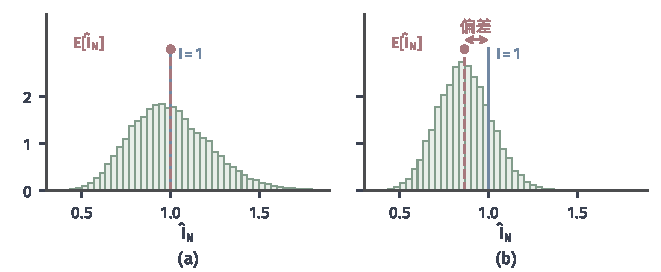
\includegraphics[width=112mm]{figures/07-probability/08-sampling-and-integration/matplotlib/mcerr-bias-spread/figure.pdf}
 \caption{估计$\mathbb{E}[X]$，$X\sim\operatorname{Exp}(1)$，每次用$N=20$个样本，重复$20000$次（种子$3101$）。绿色直方图为$\hat{I}_N$的分布，蓝线为$I=1$，红色虚线与红点为$\hat{I}_N$的平均。(a)精确的逆分位数程序；(b)把输出截到$2$的程序，红色箭头为偏差$-\mathrm{e}^{-2}$。}
 \label{fig:mcerr-bias-spread}
\end{BookInlineFigure}
